\documentclass[aspectratio=169]{beamer}
\usepackage[utf8]{luainputenc}
\usepackage[TS1,T1]{fontenc}
\usepackage{babel}
\usetheme[pagenum,navbar,ddc]{tud}
\usepackage{xcolor}
\usepackage{listings}
\usepackage{tikz}
\usepackage{caption}
\usepackage{subcaption}
\usepackage{hyperref}
\usepackage{wrapfig}
\usepackage{float}
\usepackage{pifont}
\usepackage{listings}

\hypersetup{
    colorlinks=false,
    linkcolor=black,
    filecolor=magenta,      
    urlcolor=black,
}

\definecolor{mygreen}{rgb}{0,0.6,0}
\definecolor{mygray}{rgb}{0.5,0.5,0.5}
\definecolor{mymauve}{rgb}{0.58,0,0.82}

\lstset{ 
  backgroundcolor=\color{white},   % choose the background color; you must add \usepackage{color} or \usepackage{xcolor}; should come as last argument
  basicstyle=\footnotesize\ttfamily,        % the size of the fonts that are used for the code
  breakatwhitespace=false,         % sets if automatic breaks should only happen at whitespace
  breaklines=true,                 % sets automatic line breaking
  captionpos=n,                    % sets the caption-position to bottom
  commentstyle=\color{mygreen},    % comment style
  deletekeywords={...},            % if you want to delete keywords from the given language
  escapeinside={\%*}{*)},          % if you want to add LaTeX within your code
  extendedchars=true,              % lets you use non-ASCII characters; for 8-bits encodings only, does not work with UTF-8
  firstnumber=0,                % start line enumeration with line 1000
  frame=single,	                   % adds a frame around the code
  keepspaces=true,                 % keeps spaces in text, useful for keeping indentation of code (possibly needs columns=flexible)
  keywordstyle=\color{blue},       % keyword style
  language=Octave,                 % the language of the code
  morekeywords={*,...},            % if you want to add more keywords to the set
  numbers=left,                    % where to put the line-numbers; possible values are (none, left, right)
  numbersep=5pt,                   % how far the line-numbers are from the code
  numberstyle=\tiny\color{mygray}, % the style that is used for the line-numbers
  rulecolor=\color{black},         % if not set, the frame-color may be changed on line-breaks within not-black text (e.g. comments (green here))
  showspaces=false,                % show spaces everywhere adding particular underscores; it overrides 'showstringspaces'
  showstringspaces=false,          % underline spaces within strings only
  showtabs=false,                  % show tabs within strings adding particular underscores
  stepnumber=2,                    % the step between two line-numbers. If it's 1, each line will be numbered
  stringstyle=\color{mymauve},     % string literal style
  tabsize=2,	                   % sets default tabsize to 2 spaces
  title=\lstname                   % show the filename of files included with \lstinputlisting; also try caption instead of title
}

%\title[About TEE-Design and Detection of Microarchitectural Side Channel Attacks]{About TEE-Design and Detection of Microarchitectural Side Channel Attacks}
\title[System Monitoring via Hardware Performance Counter and Trusted Execution Environment Design]{System Monitoring via Hardware Performance Counter and Trusted Execution Environment Design}
\author{Pascal Scholz}
\einrichtung{Dresden University of Technology}
\institut{Institute of Systems Architecture}
\professur{Chair of Operating Systems}
\einrichtung{}
\date{November 27th, 2024}

\newcommand*\inmm[1]{\pgfmathsetmacro\inmmwert{#1 / 1mm}\inmmwert}
\makeatletter
\newcommand*\inpt[1]{\setlength\@tempdima{#1}\the\@tempdima}
\makeatother

\AtBeginSection[]{\partpage{\usebeamertemplate***{part page}}}
\begin{document}

\newcommand{\greencheck}{}%
\DeclareRobustCommand{\greencheck}{%
    \tikz\fill[scale=0.4, color=teal]
    (0,.35) -- (.25,0) -- (1,.7) -- (.25,.15) -- cycle;%
}

\maketitle

\mode<presentation>{\setbeamertemplate{page number in footline}[frame number]}

%-----------------------------------------------------------------------------------------------------------------------
\begin{frame}{Signal Contact Discovery}
    \begin{figure}
        \only<1>{\includegraphics[width=.65\textwidth]{images/intro_1.pdf}}
        \only<2>{\includegraphics[width=.65\textwidth]{images/intro_2.pdf}}
        \only<3>{\includegraphics[width=.65\textwidth]{images/intro_3.pdf}}
        \only<4>{\includegraphics[width=.65\textwidth]{images/intro_4.pdf}}
        \only<5>{\includegraphics[width=.65\textwidth]{images/intro_5.pdf}}
    \end{figure}
\end{frame}
%-----------------------------------------------------------------------------------------------------------------------
\section{Hardware Extensions}
%-----------------------------------------------------------------------------------------------------------------------
\begin{frame}{TEE Extensions in Existing Hardware}
    \begin{itemize}
        \item SGX: Costan, Victor. "Intel SGX explained." {\footnotesize{IACR Cryptol, EPrint Arch (2016)}}
        \item TDX: "White Paper | Intel® Trust Domain Extensions" {\footnotesize{Intel Corporation, 2023}}
        \item AMD SEV-SNP: SEV-SNP, AMD. "Strengthening VM isolation with integrity protection and more." {\footnotesize{White Paper, January (2020): 1450-1465}}
        \item ARM Trustzone: Pinto, Sandro, and Nuno Santos. "Demystifying arm trustzone: A comprehensive survey." {\footnotesize{ACM computing surveys (CSUR) 51.6 (2019): 1-36}}
    \end{itemize}
\end{frame}
% %-----------------------------------------------------------------------------------------------------------------------
% \begin{frame}{ARM TrustZone: Standalone TEE}
%     \begin{figure}
%         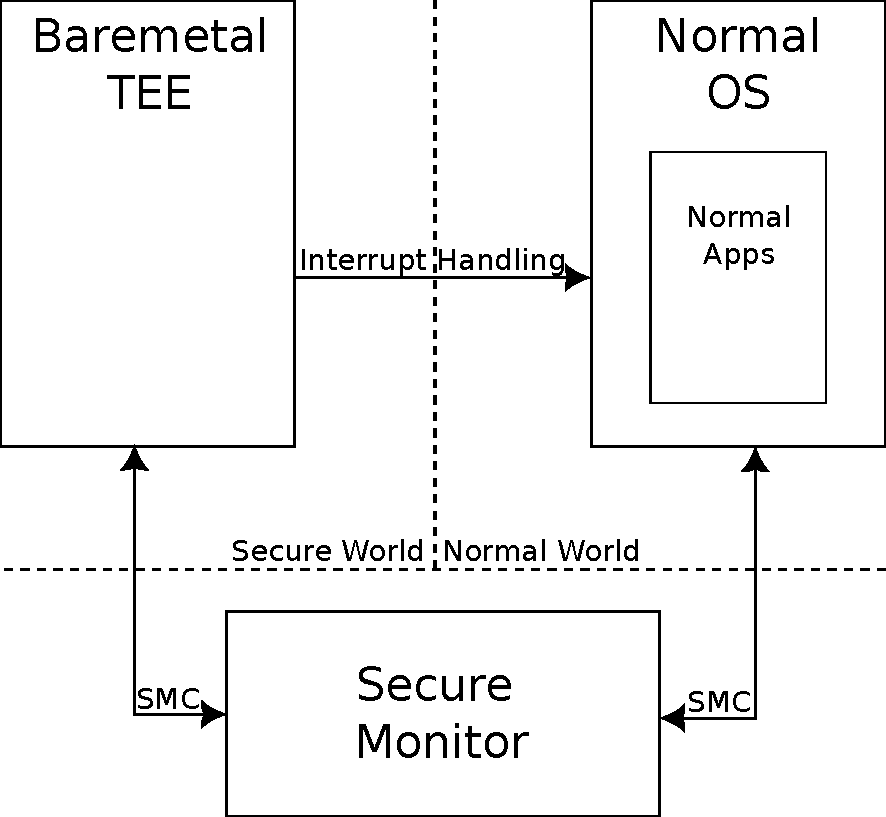
\includegraphics[width=.5\textwidth]{images/trustzone_baremetal.pdf}
%     \end{figure}
% \end{frame}
%-----------------------------------------------------------------------------------------------------------------------
\begin{frame}{ARM TrustZone: Trusted OS}
    \begin{figure}
        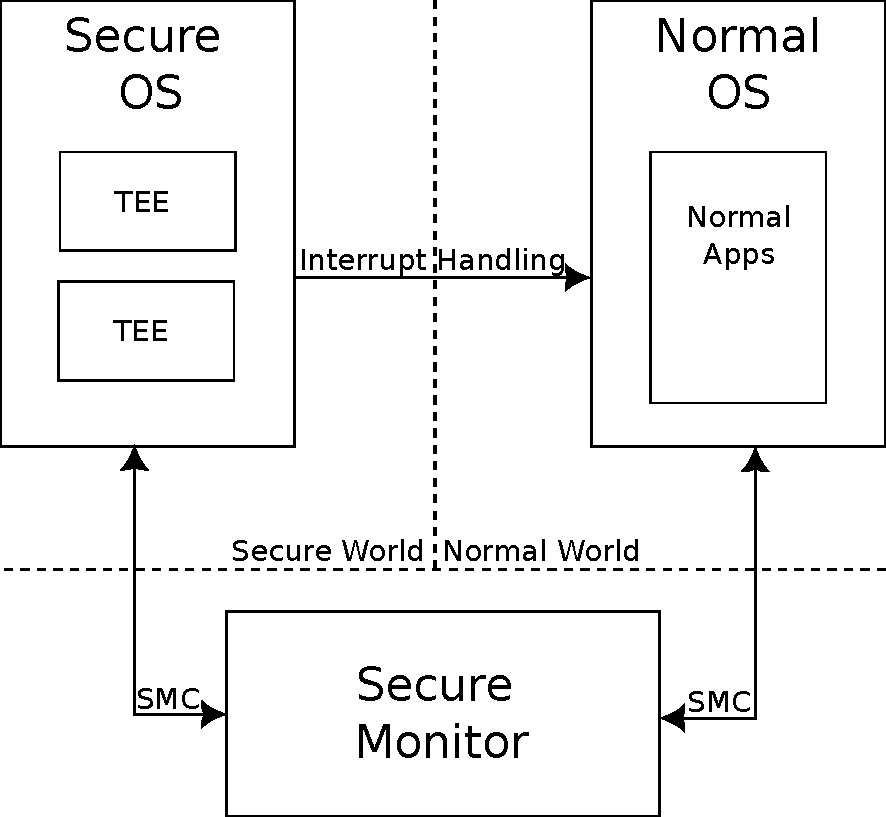
\includegraphics[width=.5\textwidth]{images/trustzone_trusted_os.pdf}
    \end{figure}
\end{frame}
%-----------------------------------------------------------------------------------------------------------------------
\begin{frame}{Intel SGX: Architecture}
    \begin{figure}
        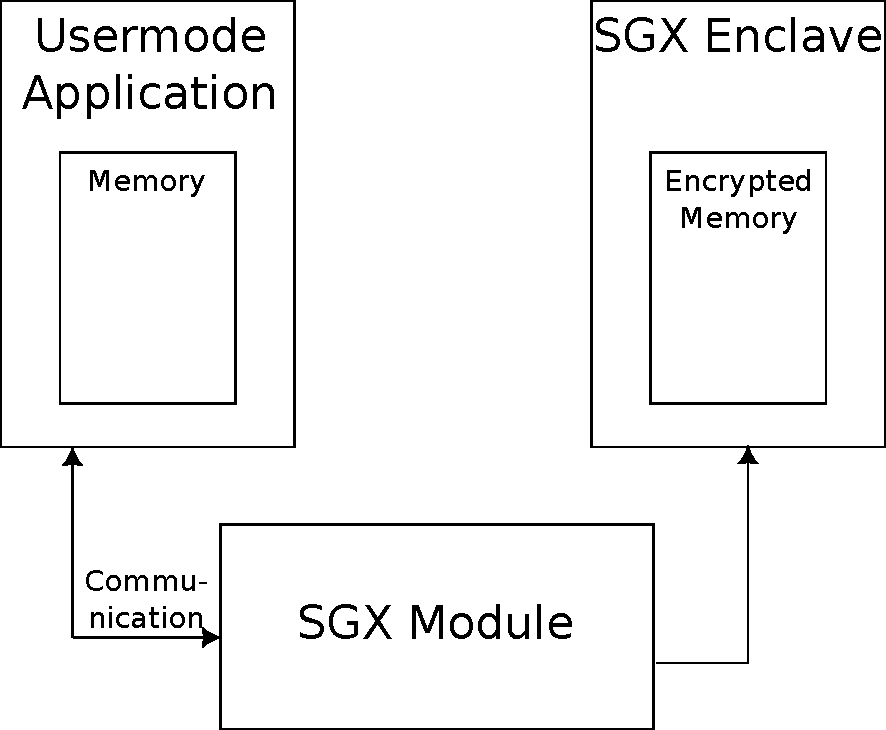
\includegraphics[width=.45\textwidth]{images/sgx_components.pdf}
    \end{figure}
\end{frame}
%-----------------------------------------------------------------------------------------------------------------------
\begin{frame}{Intel SGX: Remote Attestation}
    \begin{figure}
        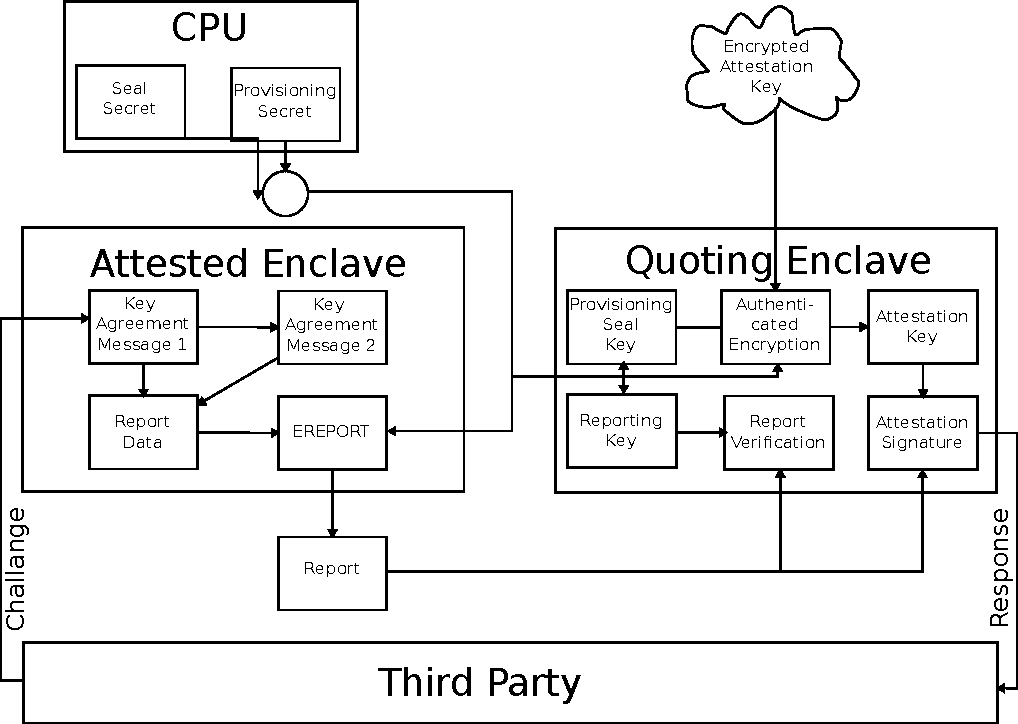
\includegraphics[width=.6\textwidth]{images/sgx_remote_attestation.pdf}
    \end{figure}
\end{frame}
%-----------------------------------------------------------------------------------------------------------------------
\begin{frame}{Intel TDX: Architecture}
    \begin{figure}
        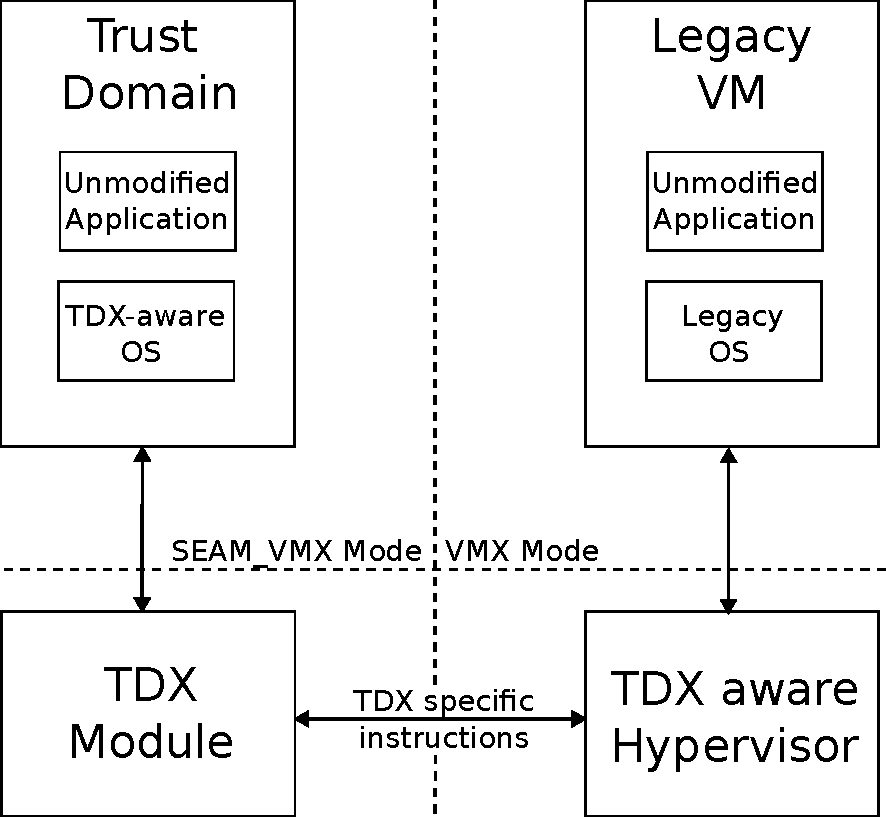
\includegraphics[width=.5\textwidth]{images/tdx_components.pdf}
    \end{figure}
\end{frame}
%-----------------------------------------------------------------------------------------------------------------------
\begin{frame}{Intel TDX: Remote Attestattion}
    \begin{figure}
        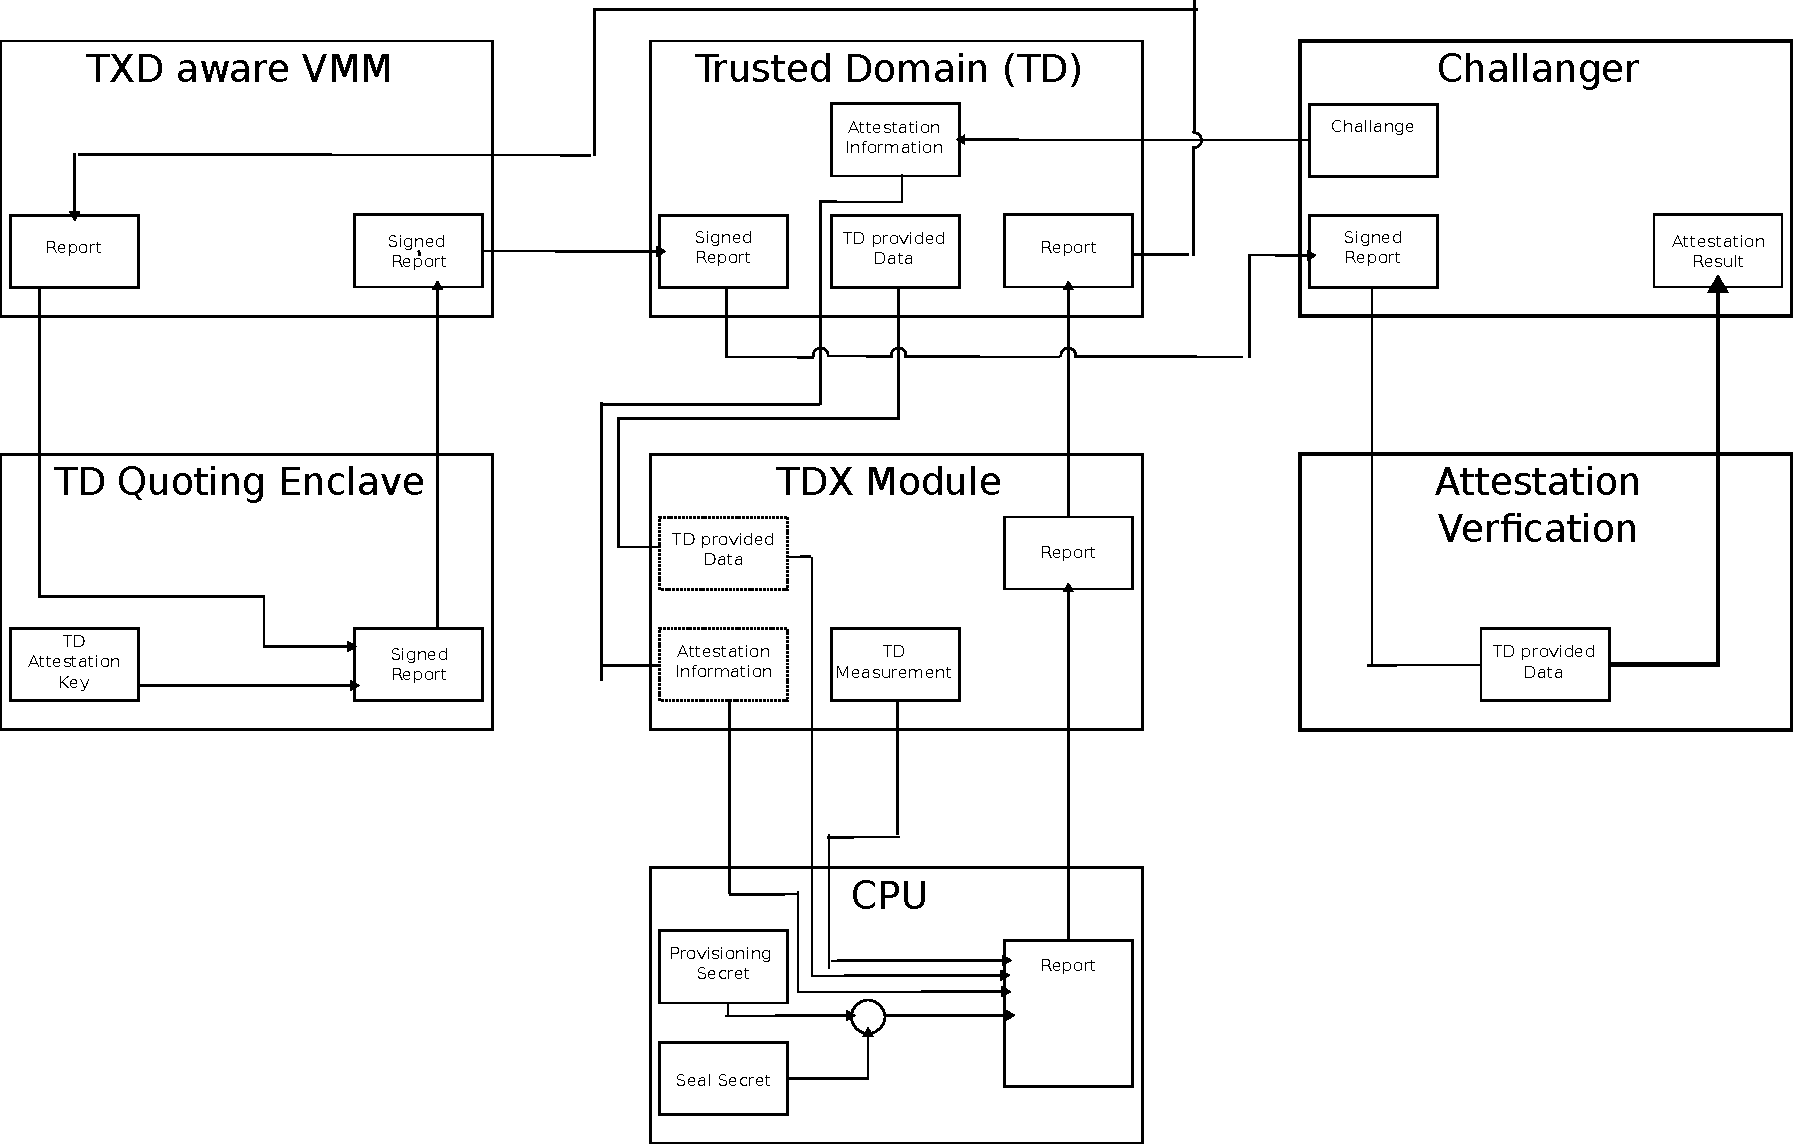
\includegraphics[width=.6\textwidth]{images/tdx_remote_attestation.pdf}
    \end{figure}
\end{frame}
%-----------------------------------------------------------------------------------------------------------------------
\begin{frame}{AMD SEV-SNP: Architecture}
    \begin{figure}
        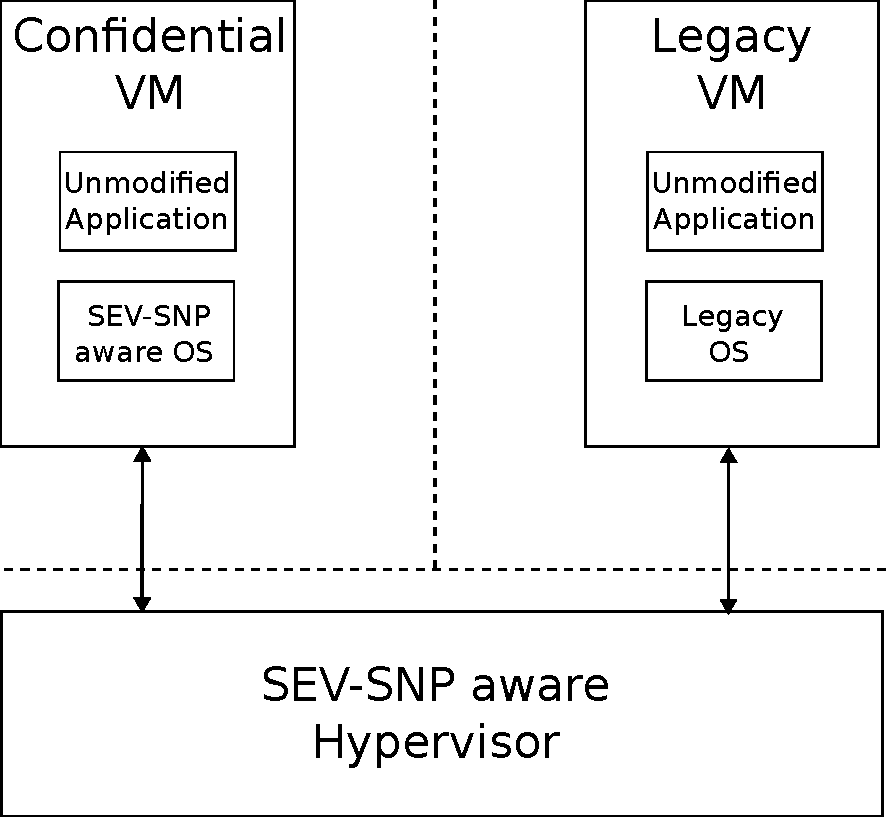
\includegraphics[width=.5\textwidth]{images/sev-snp_components.pdf}
    \end{figure}
\end{frame}
%-----------------------------------------------------------------------------------------------------------------------
\begin{frame}{AMD SEV-SNP: Remote Attestattion}
    \begin{figure}
        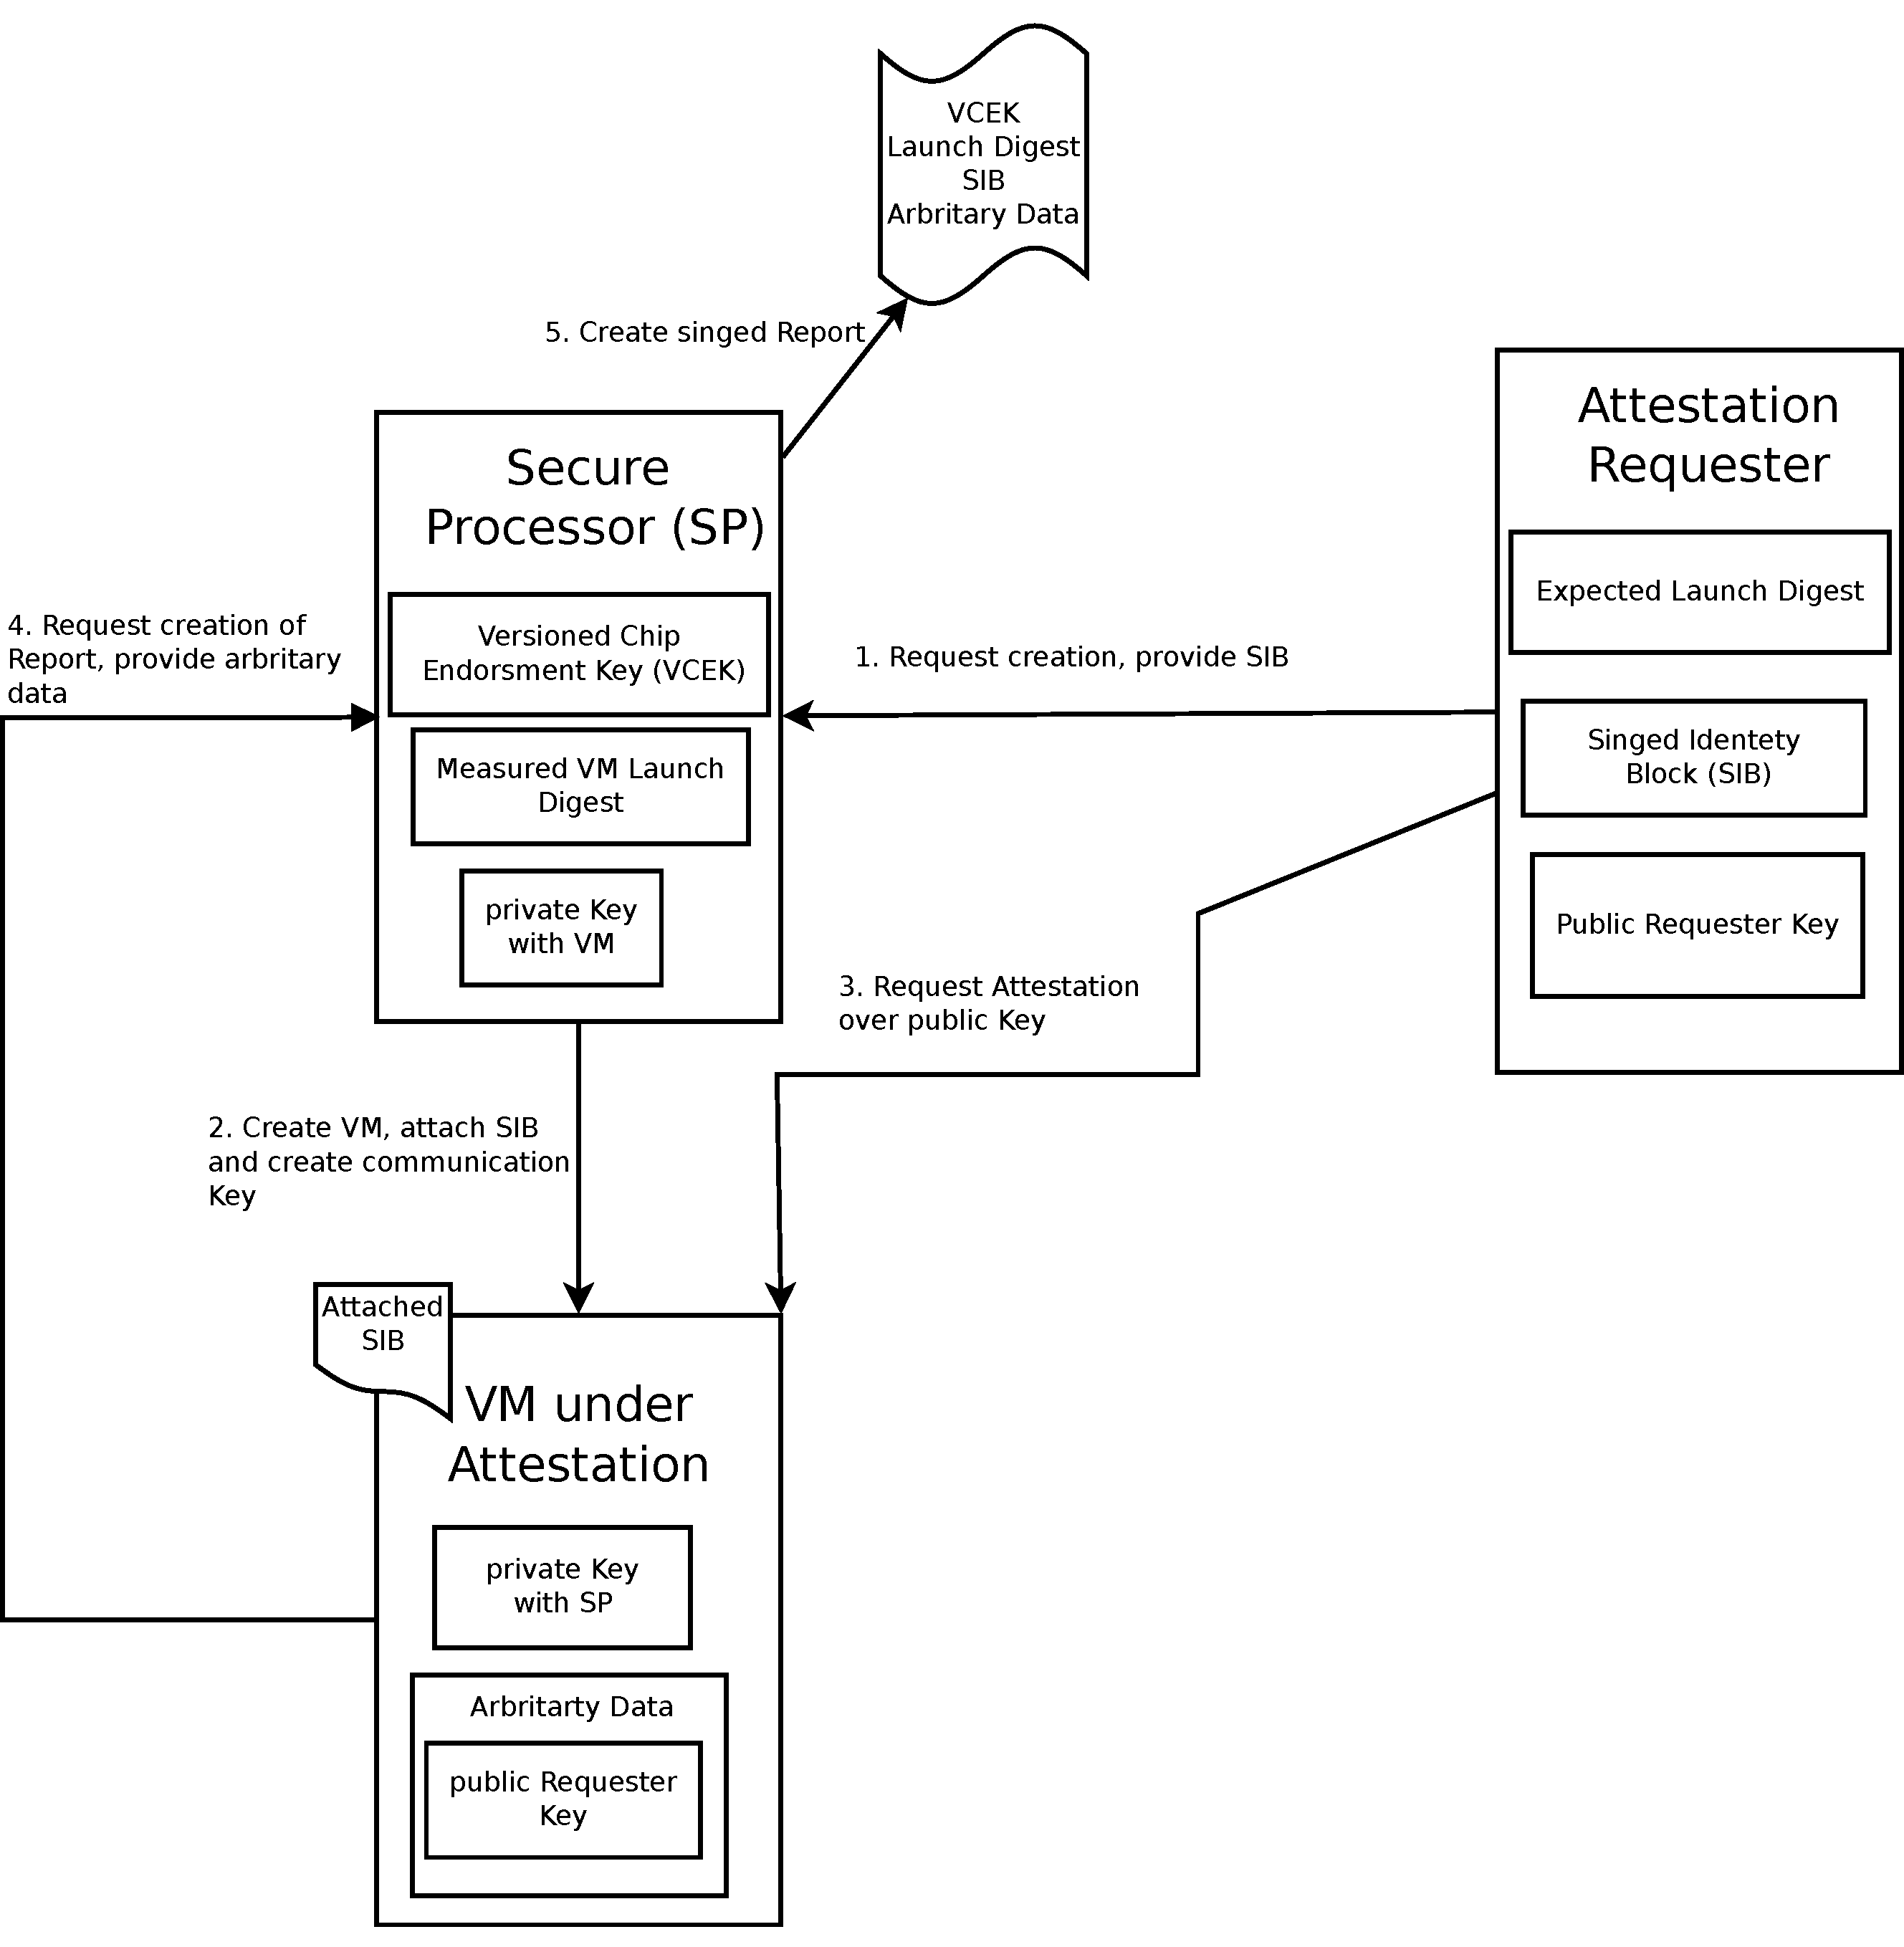
\includegraphics[width=.6\textwidth]{images/sev-snp_remote_attestation.pdf}
    \end{figure}
\end{frame}
%-----------------------------------------------------------------------------------------------------------------------
\begin{frame}{Trusted Computing Extensions: Features}
    \begin{center}
        \begin{tabular}{c|c|c|c|c}
                                         & SGX         & TDX           & SEV-SNP       & TrustZone     \\
            \hline
            Isolated Execution           & \greencheck & \greencheck   & \greencheck   & \greencheck   \\
            Remote Attestation           & \greencheck & \greencheck   & \greencheck   & (\greencheck) \\
            Memory Probing mitigation    & \greencheck & \greencheck   & \greencheck   & \ding{53}     \\
            Runs unmodified Applications & \ding{53}   & \greencheck   & \greencheck   & \greencheck   \\
            Protect against DoS          & \ding{53}   & \ding{53}     & \ding{53}     & \greencheck   \\
            Side channel mitigation      & \ding{53}   & (\greencheck) & (\greencheck) & \ding{53}     \\
        \end{tabular}\\
        \bigskip
        \greencheck - Supported \space\space\space \ding{53} - Not Supported
    \end{center}
    \bigskip
    \footnotesize{Based on: Pinto, Sandro, and Nuno Santos. "Demystifying arm trustzone: A comprehensive survey." ACM computing surveys (CSUR) 51.6 (2019): 1-36.}
\end{frame}
%-----------------------------------------------------------------------------------------------------------------------
\begin{frame}{Hardware Solutions: TCB}
    \begin{center}
        \begin{figure}
            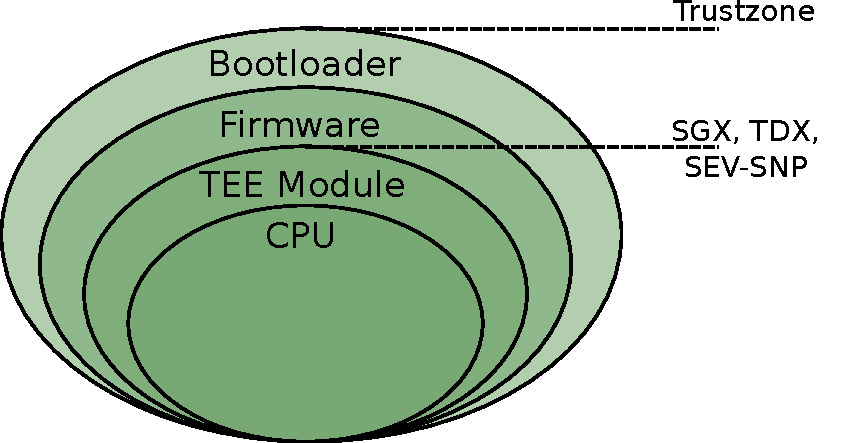
\includegraphics[width=.7\textwidth]{images/hardware_tcb.pdf}
        \end{figure}
    \end{center}
\end{frame}
%-----------------------------------------------------------------------------------------------------------------------
% \begin{frame}{Two Questions}
%     \begin{enumerate}
%         \item What about böse TEE?
%               \bigskip
%         \item What about keine Hardware in CPU?
%     \end{enumerate}
% \end{frame}
%-----------------------------------------------------------------------------------------------------------------------
\section{Software Solutions/Enhancements}
%-----------------------------------------------------------------------------------------------------------------------
\begin{frame}{Software Enclaves (Enhancements)}
    \begin{itemize}
        \item Enma: Hanna Reitz, Isolating Program Execution on L4Re/Fiasco.OC, 2019, Diploma Thesis
        \item Haven: Baumann, Andrew, Marcus Peinado, and Galen Hunt. "Shielding applications from an untrusted cloud with haven." {\footnotesize{ACM Transactions on Computer Systems (TOCS) 33.3 (2015): 1-26.}}
        \item Sice: Azab, Ahmed M., Peng Ning, and Xiaolan Zhang. "Sice: a hardware-level strongly isolated computing environment for x86 multi-core platforms." {\footnotesize{Proceedings of the 18th ACM conference on Computer and communications security. 2011.}}
    \end{itemize}
\end{frame}
%-----------------------------------------------------------------------------------------------------------------------
\begin{frame}{Haven}
    \begin{figure}
        \begin{subfigure}[]{0.45\textwidth}
            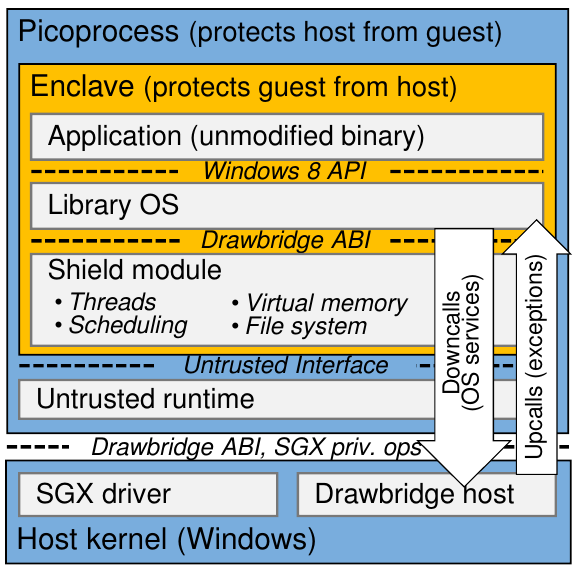
\includegraphics[width=\textwidth]{images/haven.png}
            \caption{Isolation architecture}
        \end{subfigure}
    \end{figure}
\end{frame}
%-----------------------------------------------------------------------------------------------------------------------
\begin{frame}{L4Re Enma}
    \begin{figure}
        \begin{subfigure}[]{0.6\textwidth}
            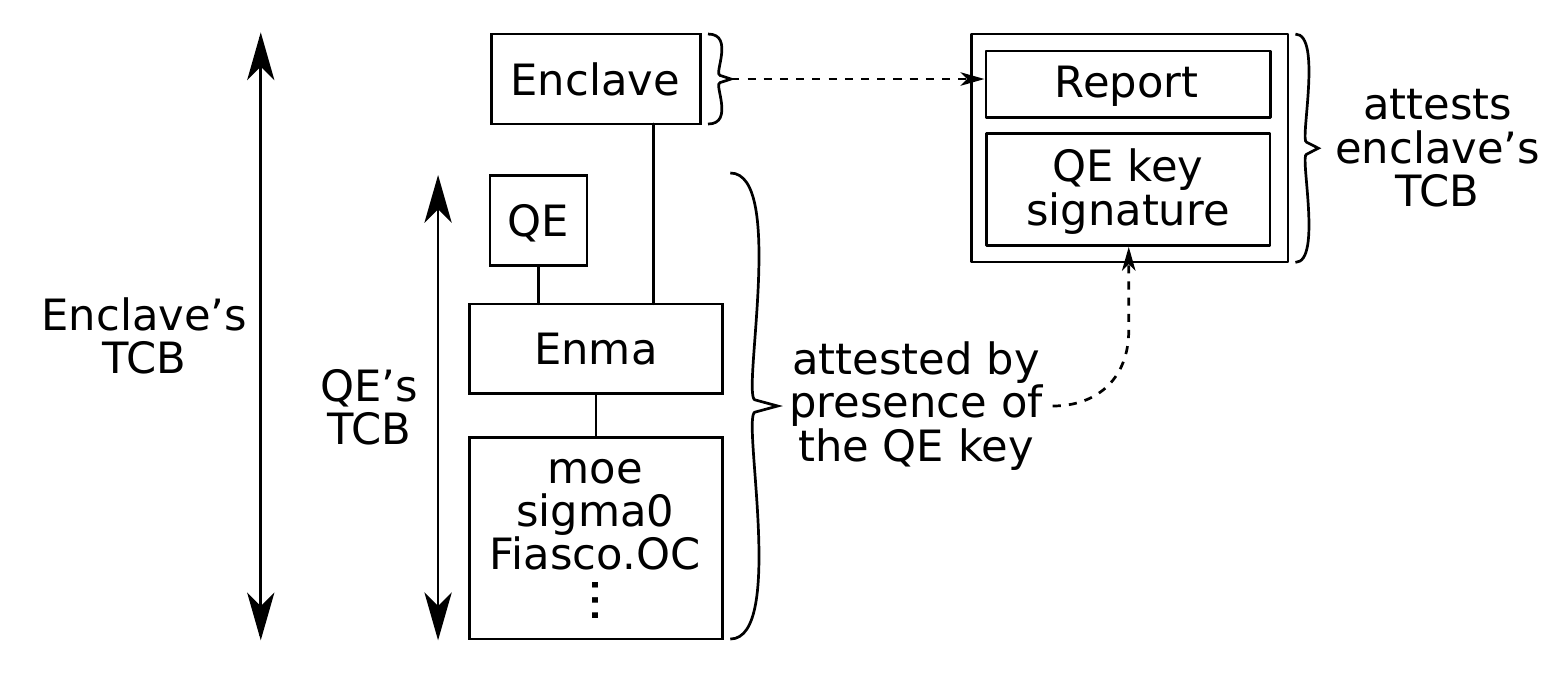
\includegraphics[width=\textwidth]{images/enma.png}
            \caption{Isolation architecture}
        \end{subfigure}
        \begin{subfigure}[]{0.35\textwidth}
            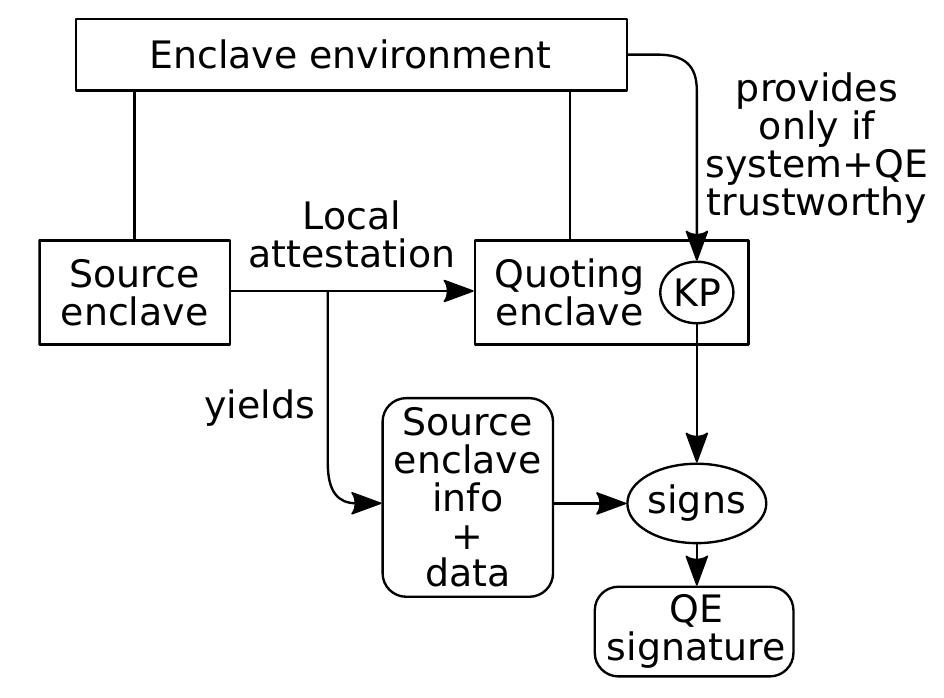
\includegraphics[width=\textwidth]{images/enma_remote_attestation.png}
            \caption{Attestation architecture}
        \end{subfigure}
    \end{figure}
    \footnotesize{Figures: Hanna Reitz, Isolating Program Execution on L4Re/Fiasco.OC, 2019, Diploma Thesis, p. 39, and p. 33}
\end{frame}
%-----------------------------------------------------------------------------------------------------------------------
\begin{frame}{Sice}
    \begin{figure}
        \begin{subfigure}[]{0.6\textwidth}
            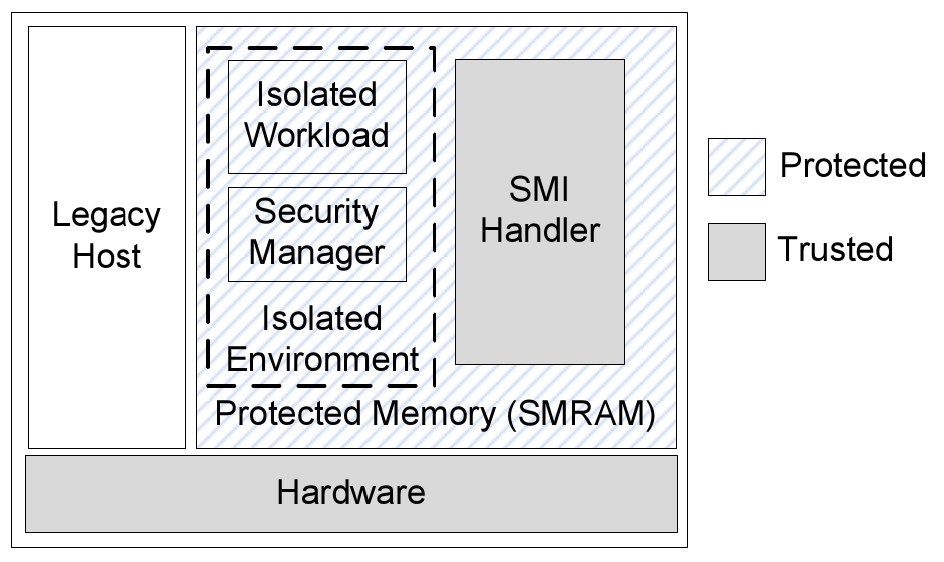
\includegraphics[width=\textwidth]{images/sice.png}
        \end{subfigure}
    \end{figure}
    \footnotesize{Figure: Azab, Ahmed M., Peng Ning, and Xiaolan Zhang. "Sice: a hardware-level strongly isolated computing environment for x86 multi-core platforms.", p. 5}
\end{frame}
%-----------------------------------------------------------------------------------------------------------------------
\begin{frame}{TCB Comparison}
    \begin{center}
        \begin{figure}
            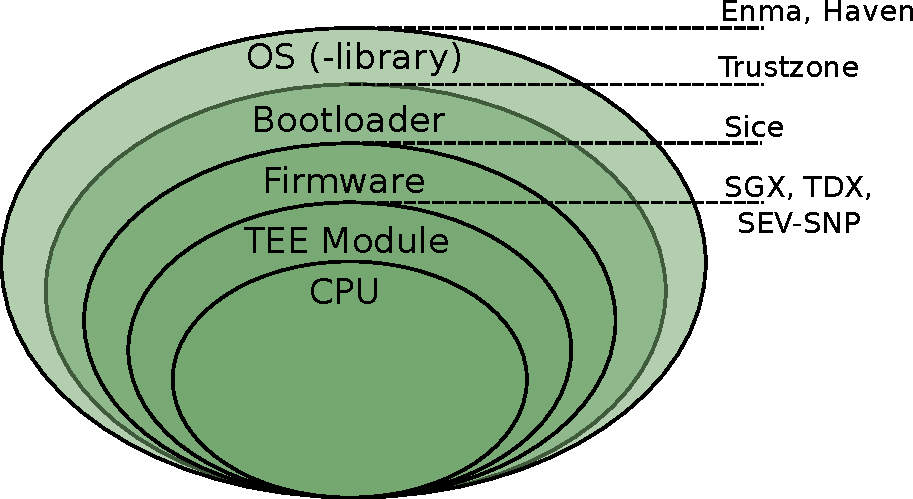
\includegraphics[width=.8\textwidth]{images/all_tcb.pdf}
        \end{figure}
    \end{center}
\end{frame}
%-----------------------------------------------------------------------------------------------------------------------
\section{Side Channel Attack Detection}
%-----------------------------------------------------------------------------------------------------------------------
\begin{frame}{Wait, Side Channel Attacks?...}
    \begin{figure}
        \begin{subfigure}[]{0.45\textwidth}
            \begin{center}
                
\includegraphics[width=0.6\textwidth]{images/spectre.pdf}
                \onslide<1>{\caption{\footnotesize{\url{https://meltdownattack.com/spectre-text.svg}, accessed 11th Nov., 2024}}}
            \end{center}
        \end{subfigure}
        \begin{subfigure}[]{0.45\textwidth}
            \begin{center}
                
\includegraphics[width=0.37\textwidth]{images/meltdown.pdf}
            \end{center}
            \caption{\footnotesize{\url{https://meltdownattack.com/meltdown-text.svg}, accessed 11th Nov., 2024}}
        \end{subfigure}
    \end{figure}
\end{frame}
%-----------------------------------------------------------------------------------------------------------------------
\begin{frame}{... How It’s Going}
    \begin{figure}
        \begin{center}
            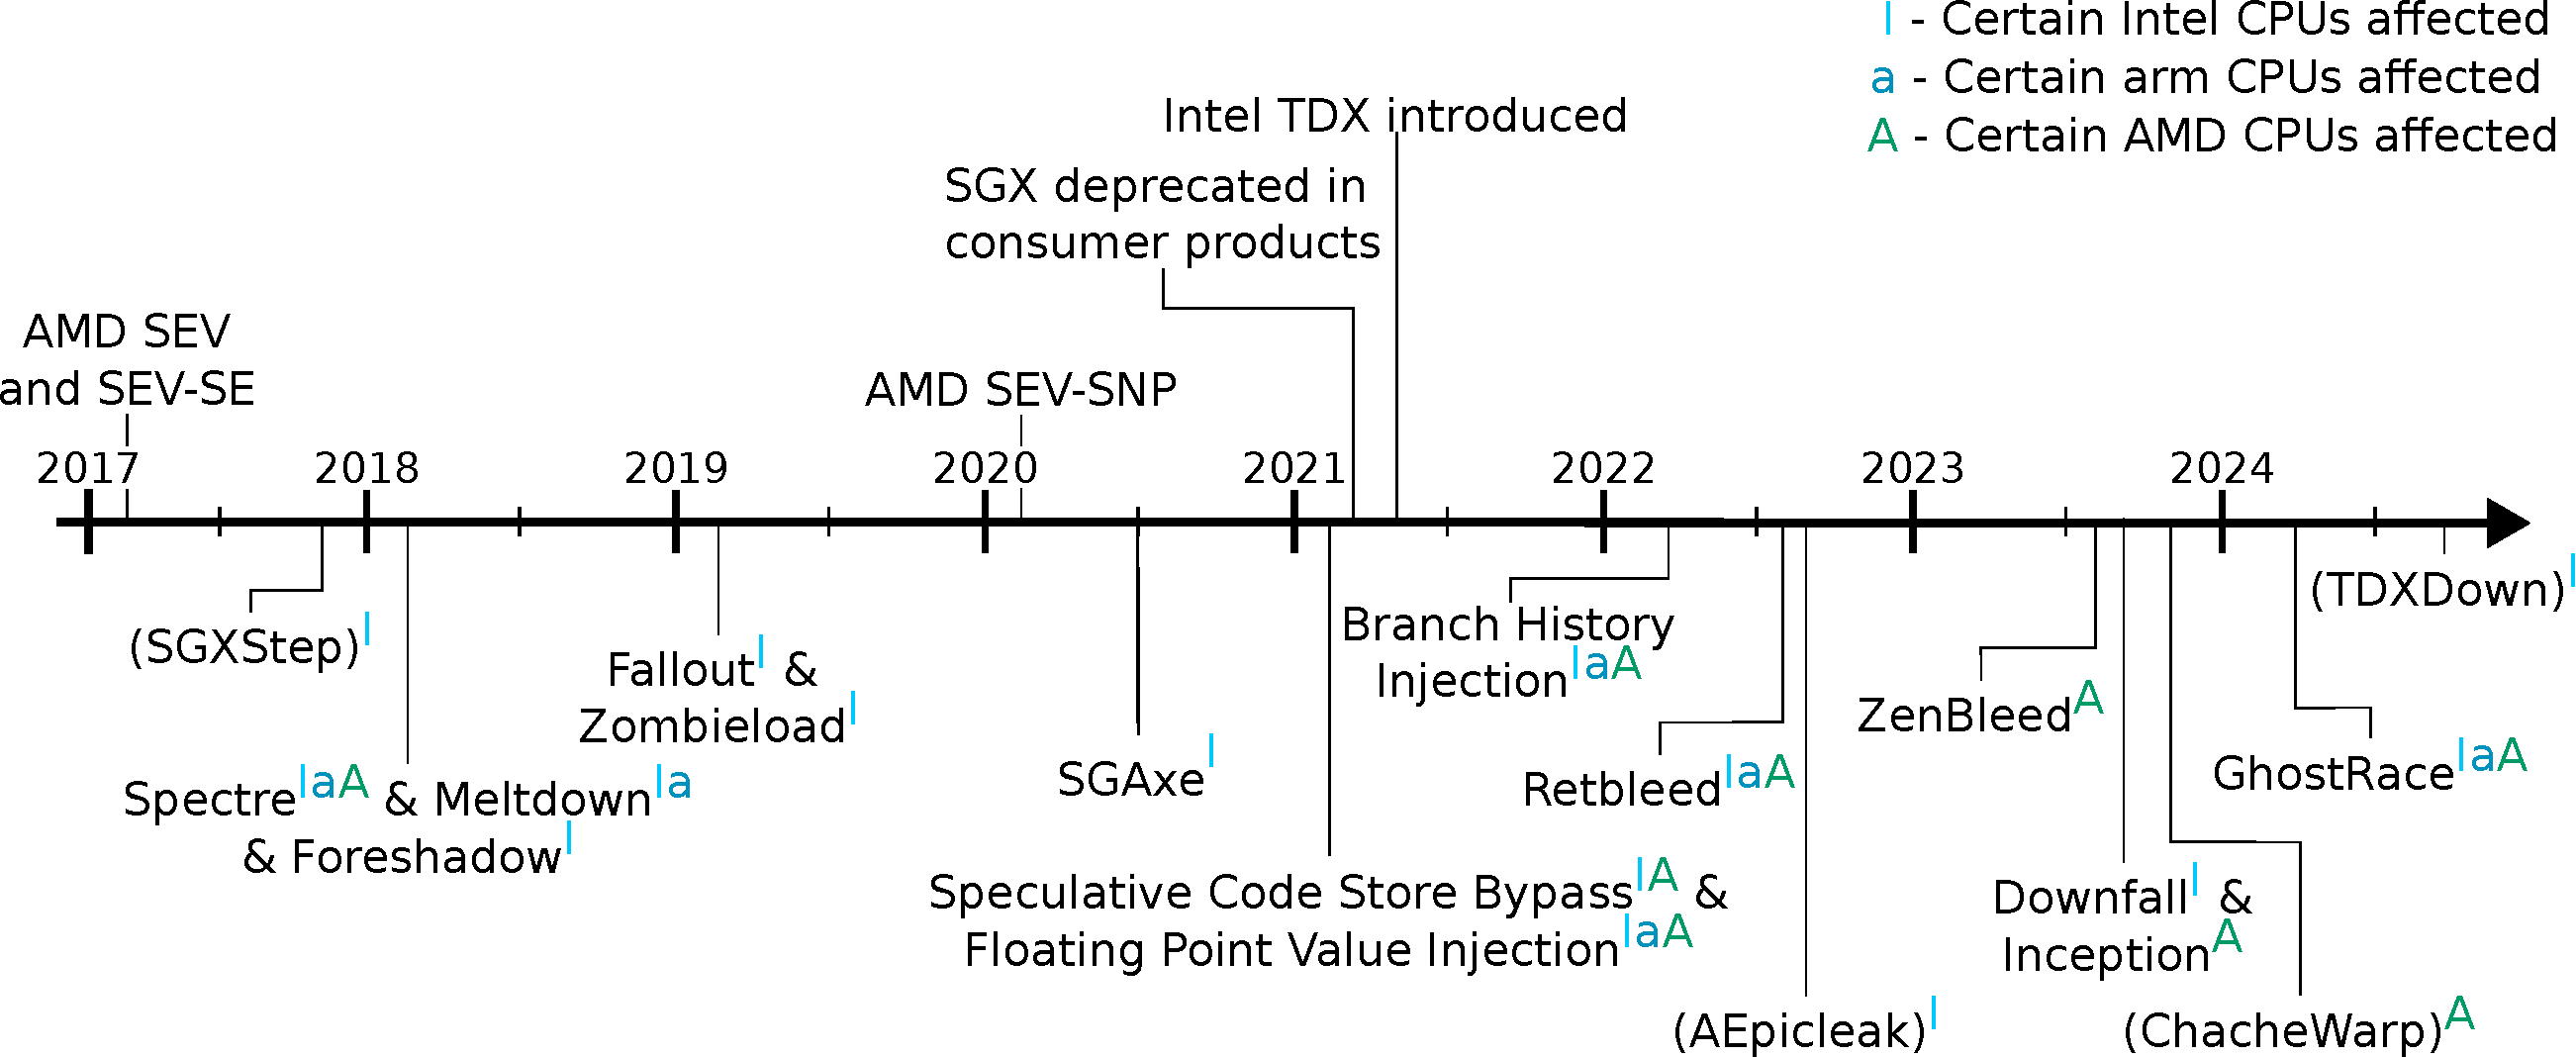
\includegraphics[width=\textwidth]{images/timeline.pdf}
        \end{center}
    \end{figure}
\end{frame}
%-----------------------------------------------------------------------------------------------------------------------
\begin{frame}{Control Flow Protection Through Performance Counters}
    \begin{itemize}
        \item CFIMon: Xia, Yubin, et al. "CFIMon: Detecting violation of control flow integrity using performance counters." {\footnotesize{IEEE/IFIP International Conference on Dependable Systems and Networks (DSN 2012). IEEE, 2012}}
        \item ConFirm: Wang, Xueyang, et al. "Malicious firmware detection with hardware performance counters." {\footnotesize{IEEE Transactions on Multi-Scale Computing Systems 2.3 (2016): 160-173.}}
    \end{itemize}
\end{frame}
%-----------------------------------------------------------------------------------------------------------------------
\begin{frame}{Hardware Performance Counters}
    \begin{minipage}{0.55\textwidth}
        \begin{itemize}
            \item Dedicated hardware Registers
            \item Used for debugging/performance analysis
            \item Can be configured to count specific event
                  \\ $\rightarrow$ profiling not only used for debugging
        \end{itemize}
    \end{minipage}
    \begin{minipage}{0.35\textwidth}
        \begin{figure}
            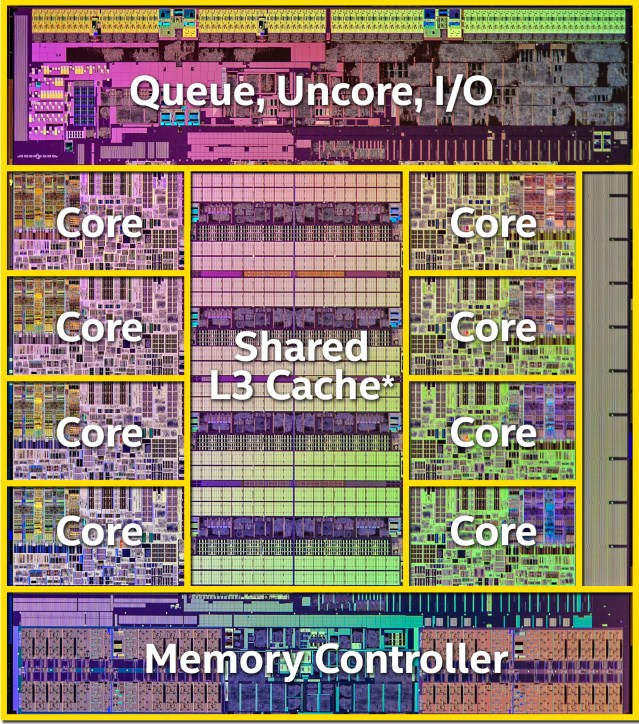
\includegraphics[width=.7\textwidth]{images/Haswell-Labeled.jpg}
        \end{figure}
    \end{minipage}\\
    \footnotesize{Figure:~\url{https://cdn.wccftech.com/wp-content/uploads/2014/12/Haswell-Labeled.jpg}, accessed 22nd, Nov., 2024}
\end{frame}
%-----------------------------------------------------------------------------------------------------------------------
\begin{frame}{Control Flow Profiling}
    \begin{center}
        \begin{minipage}{0.45\linewidth}
            \begin{center}
                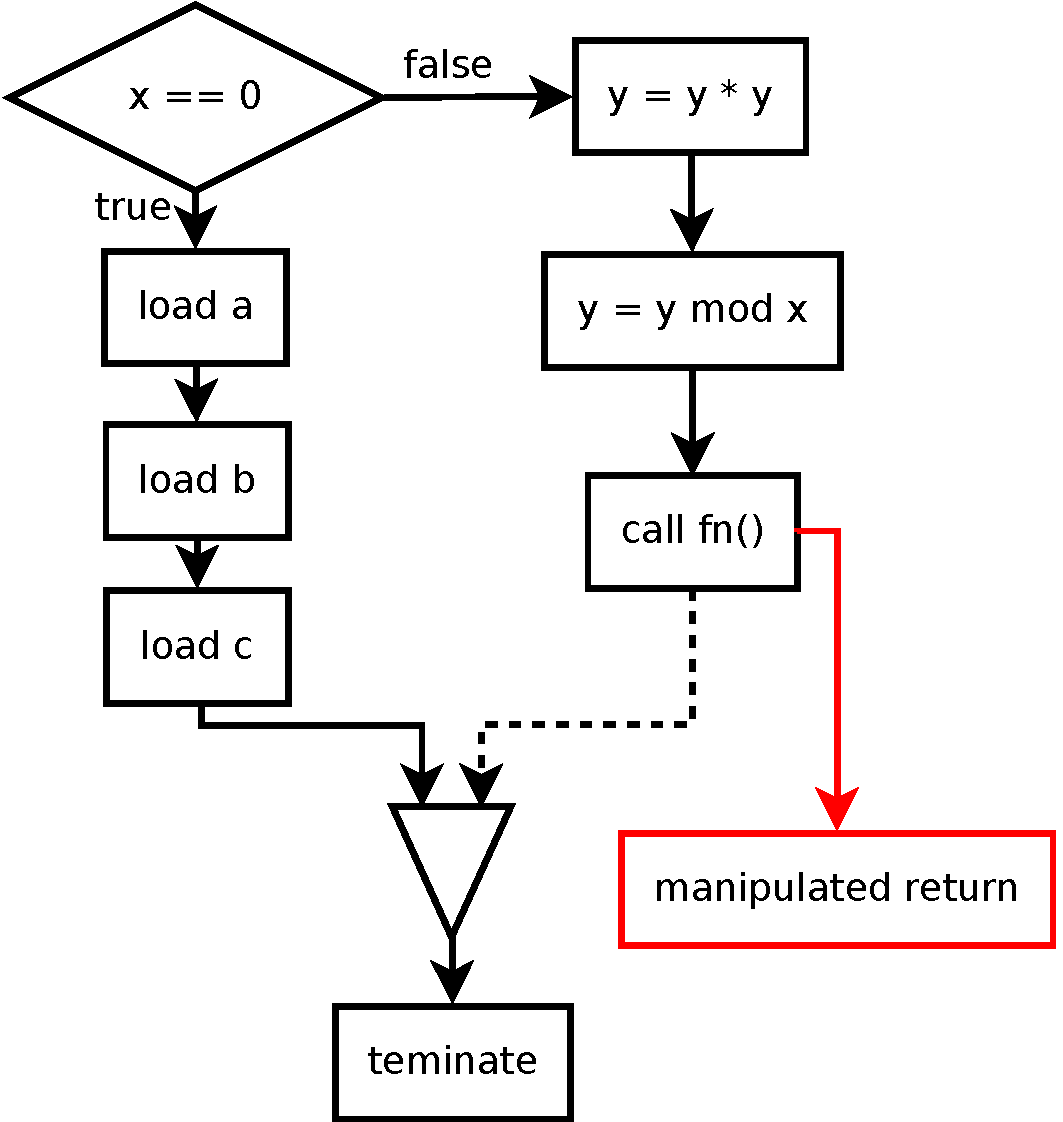
\includegraphics[width=.83\textwidth]{images/control_flow_1.pdf}
            \end{center}
        \end{minipage}
        \hfill
        \begin{minipage}{0.52\linewidth}
            \begin{center}
                \begin{tabular}{c|c|c|c}
                    Event      & Path A & Path B & Path M             \\
                    \hline
                    Loads      & 3      & 0      & 0 + {\color{red}m} \\
                    Store      & 0      & 2      & 2 + {\color{red}m} \\
                    Jump       & 0      & 1      & 1 + {\color{red}m} \\
                    Arithmetic & 0      & 2      & 2 + {\color{red}m} \\
                \end{tabular}
            \end{center}
        \end{minipage}
    \end{center}
\end{frame}
%-----------------------------------------------------------------------------------------------------------------------
\begin{frame}{Side Channel Attack Detection}
    \begin{itemize}
        \item Li, Congmiao, and Jean-Luc Gaudiot. "Detecting spectre attacks using hardware performance counters." {\footnotesize{IEEE Transactions on Computers 71.6 (2021): 1320-1331.}}
        \item Lantz, David, Felipe Boeira, and Mikael Asplund. "Towards self-monitoring enclaves: Side-channel detection using performance counters." {\footnotesize{Nordic Conference on Secure IT Systems. Cham: Springer International Publishing, 2022.}}
        \item Bazm, Mohammad-Mahdi, et al. "Cache-based side-channel attacks detection through intel cache monitoring technology and hardware performance counters." {\footnotesize{2018 Third International Conference on Fog and Mobile Edge Computing (FMEC). IEEE, 2018.}}
    \end{itemize}
\end{frame}
%-----------------------------------------------------------------------------------------------------------------------
% \begin{frame}[fragile]{Transient Execution and Side Channels}
%     \begin{center}
%         \begin{figure}
%             \begin{subfigure}[]{0.6\textwidth}
%                 \begin{lstlisting}
% if (x < array1_size)
%   y = array2[array1[x] * 4096];
%                 \end{lstlisting}
%             \end{subfigure}
%             % \begin{subfigure}[]{0.45\textwidth}
%             %     \begin{center}
%             %         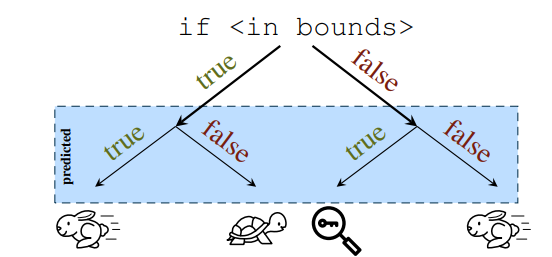
\includegraphics[width=\textwidth]{images/spectre_predict.png}
%             %         \caption{Possible predication results}
%             %     \end{center}
%             % \end{subfigure}
%             %\caption{Spectre attack mechanism: Kocher, Paul, et al. "Spectre attacks: Exploiting speculative execution." \footnotesize{Communications of the ACM 63.7 (2020): 93-101.}}
%         \end{figure}
%     \end{center}
% \end{frame}
%-----------------------------------------------------------------------------------------------------------------------
\begin{frame}{Cache Side Channel Detection}
    \begin{center}
        \begin{figure}
            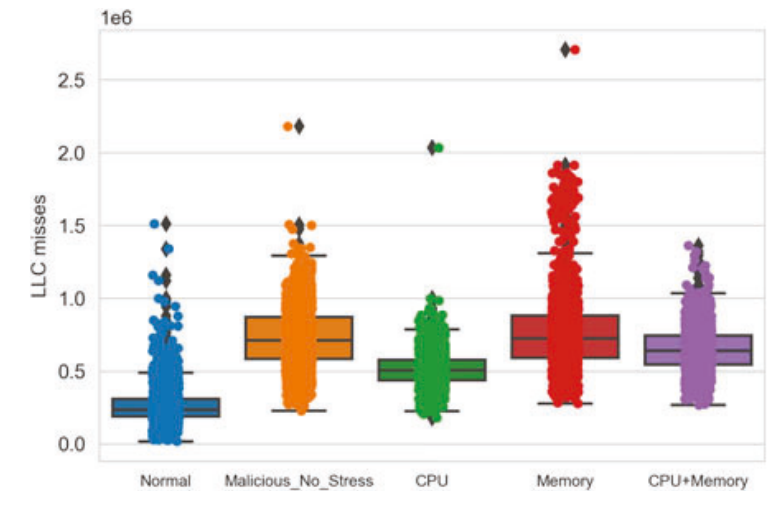
\includegraphics[width=.6\textwidth]{images/spectre_llc_miss_distribution.png}
            \caption{{\footnotesize{Li, Congmiao, and Jean-Luc Gaudiot. "Detecting spectre attacks using hardware performance counters." IEEE Transactions on Computers 71.6 (2021): 1320-1331., p. 7}}}
        \end{figure}
    \end{center}
\end{frame}
%-----------------------------------------------------------------------------------------------------------------------
\begin{frame}{LVI Attack Detection}
    \begin{center}
        \begin{figure}
            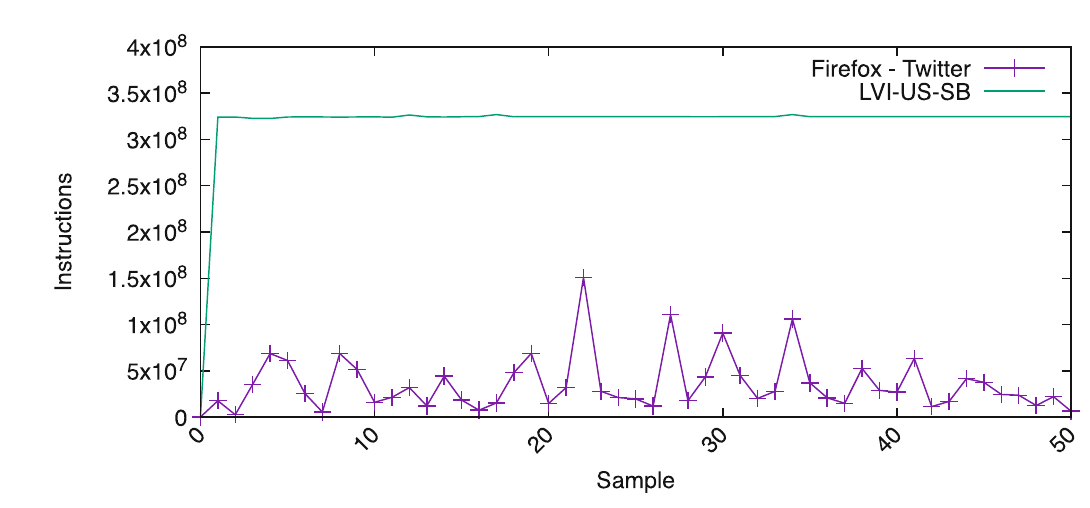
\includegraphics[width=.8\textwidth]{images/lvi_attack.png}
            \caption{\footnotesize{Lantz, David, Felipe Boeira, and Mikael Asplund. "Towards self-monitoring enclaves: Side-channel detection using performance counters." Nordic Conference on Secure IT Systems. Cham: Springer International Publishing, 2022, p. 10}}
        \end{figure}
    \end{center}
\end{frame}
%-----------------------------------------------------------------------------------------------------------------------
\begin{frame}{Spectre Attack Obfuscation}
    \begin{center}
        \begin{figure}
            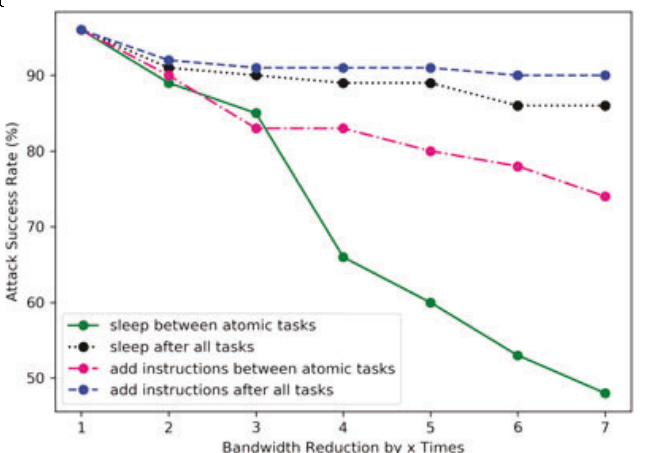
\includegraphics[width=.5\textwidth]{images/evasive_spectre.png}
            \caption{{\footnotesize{Li, Congmiao, and Jean-Luc Gaudiot. "Detecting spectre attacks using hardware performance counters." IEEE Transactions on Computers 71.6 (2021): 1320-1331., p. 7}}}
        \end{figure}
    \end{center}
\end{frame}
%-----------------------------------------------------------------------------------------------------------------------
\begin{frame}{Conclusion}
    \begin{itemize}
        \item Shared resources abused for side channels
        \item Hardware/Software still vulnerable
        \item Side channel attacks can evade detection attempts
    \end{itemize}
\end{frame}
%-----------------------------------------------------------------------------------------------------------------------
\begin{frame}{No Medium, No Channel}
    \begin{itemize}
        \item Idea: No side channel medium $\rightarrow$ no side channels
        \item Proposed with QuanShield\footnote{Cui, Shujie, et al. "QuanShield: Protecting against Side-Channels Attacks using Self-Destructing Enclaves." arXiv preprint arXiv:2312.11796 (2023).}\\
              $\rightarrow$ No Interrupts $\rightarrow$ No interrupt-based side channels
    \end{itemize}
\end{frame}
%-----------------------------------------------------------------------------------------------------------------------
\begin{frame}{Open Research: Restriction of Shared Resources}
    Open Question: How far can we go when restricting shared resources?
    \bigskip
    \begin{minipage}{0.55\textwidth}
        \begin{itemize}
            \item Isolate software strictly to one core
            \item Don't use shared parts of memory system
            \item Enforce isolation using Performance Counter (or similar)
        \end{itemize}
    \end{minipage}
    \begin{minipage}{0.35\textwidth}
        \begin{figure}
            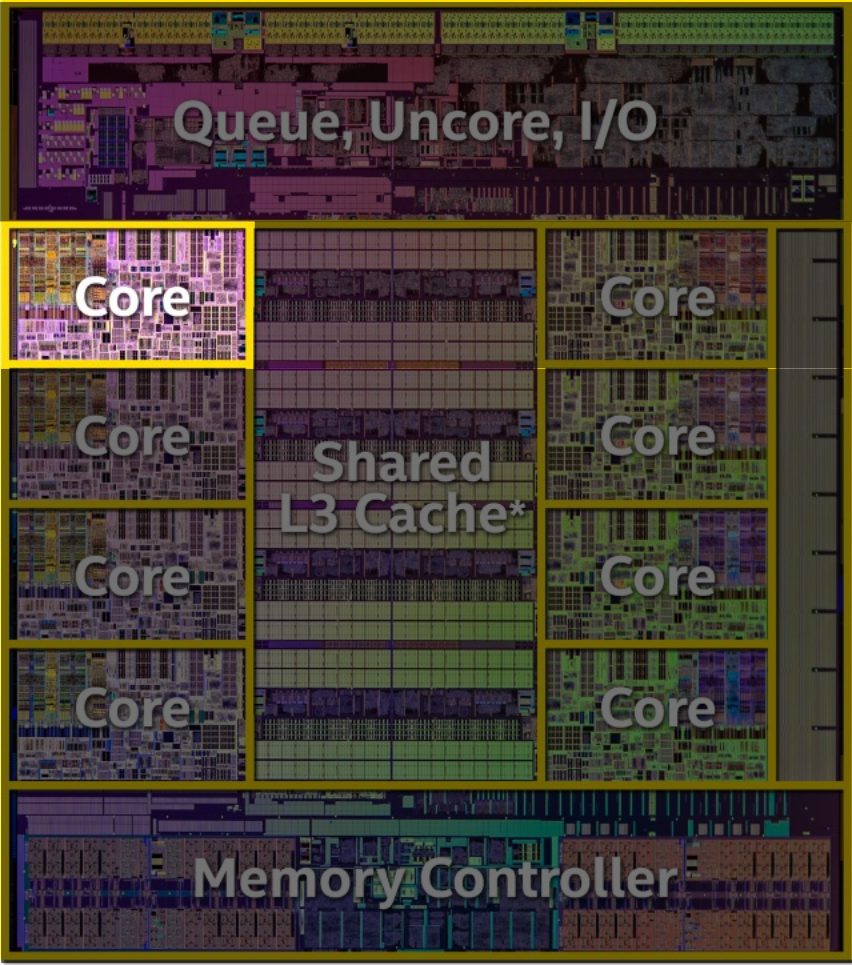
\includegraphics[width=.7\textwidth]{images/haswell_labeled_core.png}
        \end{figure}
    \end{minipage}\\
    \footnotesize{Figure:~\url{https://cdn.wccftech.com/wp-content/uploads/2014/12/Haswell-Labeled.jpg}, accessed 22nd, Nov., 2024}
\end{frame}
%-----------------------------------------------------------------------------------------------------------------------

\end{document}
